\documentclass[12pt,fleqn]{article}\usepackage{../../common}
\begin{document}
Risk ve Oynaklık Hedeflemesi

En basit formunda risk idaresi için risk eşliği yöntemi (risk parity) var;
enstrümanlara portföyde risklerine (oynaklıklarına) ters oranda ağırlık
vermek. [1] buna bazı ekler yapar, bir oynaklık hedefi kavramını ekler ve bu
hedefe göre her alt sistemi ayarlar. Ayrıca risk eşliği oynaklığı bir kez
hesaplar ve bir daha bakmaz, yeni sistem oynaklığı her gün belli gün geriye
bakarak tüm enstrümanlar için tekrar tekrar hesaplar.

Hedefleme şöyle işler: Önce bir yıllık oynaklık yüzdesi hedefleriz, yüzde 20
diyelim, ve bu yüzdeden bir nakit oynaklık hedefi hesaplarız. Sermaye 100,000
lira için bu 20,000 lira, bunu gün seviyesine indiririz, 20,000 / $\sqrt{256}$ =
1,250. Ardından her enstrümanın günlük fiyat oynaklığını buluruz, ve günlük
oynaklık bölü bu sayı ile o enstrümandan kaç tane alacağımızı hesaplarız. Bu
konunun detaylarını işleyeceğiz. Diğer her parametre bu hedefe göre
değiştirilir. Bu yaklaşımın iyi tarafı yatırımcı kendini rahat hissettiği, ve
getirisini yeterli bulduğu bir oynaklık üzerinde önceden karar verir, ve
portföyünü buna göre düzenler, ve bu oynaklık bir daha (uzun süre) değişmez.

Sharpe oranı (SO) ile oynaklık hedeflemesi arasında bir ilişki var. Önce şunu
belirtelim, bu yaklaşımda kazanç ile sermaye artmış ise o zaman oynaklık yüzdesi
ile daha çok para yatırıma gitmelidir, kayıpta daha az. Bu da daha önce
gördüğümüz Kelly yaklaşımının bir çeşidi. Şimdi, oynaklığı SO ile çarparak
yıllık beklenen getiriyi hesaplamak mümkündür, çünkü SO zaten getiri bölü risk,
yani bölü oynaklık idi.

Blok Degeri

Bir enstrümanın blok değeri o enstrümanın en ufak biriminde, o enstrümanın
fiyatının \%1 değişmesi ile ortaya çıkan fiyat farkıdır. Mesela ham petrol
vadeli işlem sözleşmelerinde 1 kontraktın içinde 1000 varil vardır. Eğer yüzde 1
değişim ile fiyat \$75'ten \$75.75'e çıkarsa tüm değişim \$.75 * 1000 = \$750
demektir. Blok değeri budur. 

Fakat yüzde 1'lik değişimin şansı nedir? Senetlerin ortalama fiyat oynaklığı
yüzde 1 olabilir, diğer yanda Almanya 2-yıllık Schatz tahvil VİS'lerinin günlük
standart sapması \%0.02'dır. Petrole dönelim, diyelim ki tarihi veriye bakarak
günlük ortalama değişimin yüzde 1.33 olduğunu bulduk, bu durumda günlük kar veya
kaybımız ortalama 750 Dolar x 1.33 = 997.50 Dolar olacak demektir, çünkü yüzde
1'lik değişim 750 Dolar idi. Bu sonuca enstrüman kur oynaklığı (instrument
currency volatility) diyelim.

Bir adım daha, eğer portföyümüz Türkiye'de TL bazlı bir hesap kullanıyorsak, kur
değişimi yapmamız lazım, bu örnek için İngiliz pound olsun, USD/GBP kuru bugün
0.67, o zaman 997.50*0.67 = 668.325 Pound.

Formül yerine tek bir değer kayıtlı tutmak daha rahat olduğu için bir tek sayı
değeri de hesaplanabilir, nokta değeri (point value) burada kullanılır; bir
VİS'in fiyatında 1 birimlik değişimin ne kadar toptan değişimi temsil ettiği
yani. Üstteki petrol örneğinde \$1'lik degisim kontraktta 1000 varil olduğu için
bu \$1000'lik bir değişim demektir, nokta değeri olarak bu tutulur. Günlük
ortalama yüzde değişimi biliyoruz zaten, 75 x 0.0133 x 1000 = 997.50 Dolar. Aynı
sonuca eriştik.

Bu sayı bir enstrümanlık bloğu elde tutmanın günlük riskini gösteriyor, yani tek
bir VİS. Eğer portföyde sadece bu entsruman olsaydı, ve 1,000,000 Pound yıllık
oynaklık hedefimiz olsaydı, günlük hedef için $\sqrt{256}$'ya bölüyoruz, yani
1/16'sı 62,500 Pound olur. Bu günlük oynaklık kapasitemiz içine kaç tane petrol
VİS'i sığdırabilirdik? Bunun için kapasitemizi günlük tek enstrüman petrol
riskine bölüyoruz, 62,500 / 668.325 = 93.52 tane kontrakt. Dikkat bu noktaya
kadar hiç yuvarlama yapmadan geldik. Bu arada dikkat edildiyse, bu risk doldurma
işlemini sanki oynaklık hedefinin elverdigi tüm parayı sadece o alt sistemde
harcayabilirmişiz gibi yapıyoruz. Daha sonra her alt sisteme ayrılan yüzde ile
çarpınca paylaştırma tam yapılmış oluyor. Ama bu adım sonra geliyor.

Harcamalar (Costs)

Eğer herhangi bir bir enstrüman için o enstrümandan tek bir bloğu alıp hemen
satsaydım, bu git/gel'in o enstrümanın yıllık riskine oranlı bedeli ne olurdu?
Bu "standardize edilmiş bedel" bize her git/gel'in yıllık bazlı Sharpe oranından
ne kadar kaybettireceğini bize söyler. Sharpe oranı bildiğimiz gibi getirinin
yıllık oynaklığa bölünmüş halidir, getirinin oynaklığa olan oranı yani,
standardize edilmiş bedel de benzer bir hesabı yapar, böylece elde ettiğimiz
bedeli direk Sharpe oranından çıkartabilmemizi sağlar.

Git / gel dedik, yani bu ilk harcamanın hesabı alış fiyatı / satış fiyatı
aralığıyla yapılır. Niye? Çünkü aldığımızda alış, sattığımızda satış fiyatından
satıyoruz. Dikkat: geriye dönük testlerde bir fiyat kullandığımızda bu fiyat
çoğunlukla AFSF iki uç noktasının tam orta noktasıdır; Fakat ya orta noktadan
alım, ya da satım yapamadıysak?  İşte bu ``en kötü ihtimal'' bize bir masraf
olarak yansır, ki her zaman bu en kötü ihtimale göre bir harcama kalemini hesaba
katmamız gerekir. O zaman ASFS yayılımını (spread) buluruz, ve ikiye böleriz, bu
harcamadır.

AFSF nereden elde edilir?  Borsa aracımızın sağladığı araç üzerinden enstrümanın
en son AFSF'na bakarız, ve (birazdan göreceğimiz şekilde) masrafı Sharpe oranına
oranlı hesaplarız, bu sebeple hacimden, oynaklıktan ileri gelen değişimlere
uyarlanmış bir hesap elde etmiş oluruz.

Geçmişte, tarihi verideki her günde AFSF'nin ne olduğu çoğunlukla kaydedilen ve
paylaşılan bir veri değildir, ama illa ki gerekiyorsa, onu tahmin edebilen bazı
metotlar mevcut, bkz {\em Ekler} bölümü.

Neyse, araca gireriz, vadeli işlem sözleşmeleri için bir kerede kaç tane
sözleşme alınacağı AFSF için bir eşik değeri oluşturabilir, buna da dikkat,
mesela Euro Stoxx 50 için Ocak 23, 2015'te bakıyoruz, 437 sözleşme ve altındaki
satımlar için 3369 fiyatı verilmiş, alımlarda 7 sözleşme ve altı alımlar için
3370 fiyatı verilmiş. Harcama demek ki 3370-3369 / 2 = 0.5 (altta
\verb!slippage! kolonunda). Şimdi bu bedeli yine en son fiyata göre bir yüzdeye
çeviririz, 0.5 / 3370 * 100 = \%0.01483. Ardından bu değeri bir para miktarına
çeviririz, yüzde 1'lik değişimi temsil eden değer 3370 fiyat seviyesinde 337 Eur
eder (3370 * nokta değeri * yüzde 1, yani 3370 * 10/100). 337 çarpı 0.0148 = 5
Eur.

Borsa aracı şirketi ek bazı masraflar kesebilir, bu örnekte her sözleşme için 3
Eur kesiliyor mesela.

Sharpe oranıyla alakalı bir bedel oluşturma yönünde ilerliyoruz.  Çıkartma
işlemini şöyle yaparız; bir sene içinde bu enstrümanı, bir tanesini, sadece bir
kez ardı ardına al/sat yaptıysak bu blok masraf C = 5 + 3 = 8 Eur üzerinden 2 *
C eder. Diyelim Euro Stoxx enstrüman oynaklığı günlük yüzde 1.5, her yüzde 1'lik
hareket 370 Eur ediyor, 370 * 1.5 = 506 Eur, bu günlük standart sapma. Onu
yıllık standart sapma haline getirmek için 506 * 16 = 8096 Eur.  2 * 8 /8096 =
0.002 SO ünitesi. Yani bu değer artık SO'dan çıkartabileceğimiz bir sayıdır.

\begin{minted}[fontsize=\footnotesize]{python}
import pandas as pd
from StringIO import StringIO

COSTS=u"""
instrument,currency,point_value,slippage
CRUDE_W,USD,1000,0.0145328653
EDOLLAR,USD,2500,0.0025
US5,USD,1000,0.004
EUROSTX,EUR,10,0.5
V2X,EUR,100,0.0255
MXP,USD,500000,0.000011567
CORN,USD,50,0.125
"""
costs = pd.read_csv(StringIO(COSTS),index_col=0)

my_curr = 'USD'
vol_target = 0.20
capital = 250*1000
exchange = {'USD': {'EUR': 1.1, 'USD': 1.0} }
daily_vol_target = capital * vol_target / 16

def calc_cost(ins,dt = '2014-10-14'):
    with zipfile.ZipFile('legacycsv.zip', 'r') as z:
        dfi = pd.read_csv(z.open('%s_price.csv' % ins), index_col=0,parse_dates=True )
        vol = pd.rolling_std(dfi.pct_change()*100., window=25)    
    res = []
    price = float(dfi.ix[dt])
    v = float(vol.ix[dt])
    point_val = price * costs.ix[ins].point_value / 100.
    block_vol = block_val*v
    inst_value_vol =  block_vol*exchange[my_curr][costs.ix[ins].currency]
    units = daily_vol_target / inst_value_vol
    exec_cost = (costs.ix[ins].slippage / price) * 100 * block_val
    so_cost =  (exec_cost * 2.) / (16. * block_vol)
    return price,v,block_val,block_vol,inst_value_vol,units,exec_cost,so_cost

price,v,block_val,block_vol,inst_value_vol,units,exec_cost,so_cost = calc_cost('EUROSTX')
print so_cost
\end{minted}

\begin{verbatim}
0.001862369503
\end{verbatim}


\begin{minted}[fontsize=\footnotesize]{python}
import pandas as pd, zipfile
from io import StringIO
pd.options.display.float_format = '{0:.4f}'.format    

instruments = ['CRUDE_W','EDOLLAR','US5','EUROSTX','V2X','MXP','CORN']
         
dt = '2014-10-14'
res = []
cols = ['inst','price','v','block_val','block_vol','inst_value_vol','units','exec_cost','so_cost']
for inst in instruments:
    price,v,block_val,block_vol,inst_value_vol,units,exec_cost,so_cost = calc_cost(inst)
    res.append([inst,price,v,block_val,block_vol,inst_value_vol,units,exec_cost,so_cost])
    
print pd.DataFrame(res,columns=cols)         
\end{minted}

\begin{verbatim}
      inst     price      v  block_val  block_vol  inst_value_vol   units  \
0  CRUDE_W   85.3000 1.2678   853.0000  1081.4529       1081.4529  2.8896   
1  EDOLLAR   97.0550 0.0563  2426.3750   136.7107        136.7107 22.8585   
2      US5  117.0625 0.1699  1170.6250   198.9413        198.9413 15.7081   
3  EUROSTX 2816.0000 1.1917   281.6000   335.5940        369.1534  8.4653   
4      V2X   22.8000 2.6898    22.8000    61.3265         67.4592 46.3243   
5      MXP    0.0718 0.5110   358.7500   183.3214        183.3214 17.0466   
6     CORN  422.7500 1.2475   211.3750   263.6875        263.6875 11.8511   

   exec_cost  so_cost  
0    14.5329   0.0017  
1     6.2500   0.0057  
2     4.0000   0.0025  
3     5.0000   0.0019  
4     2.5500   0.0052  
5     5.7835   0.0039  
6     6.2500   0.0030  
\end{verbatim}

Devir (Turnover)

Tabii SO'dan çıkartma yapmadan önce bir enstrümanı senede yaklaşık kaç kez alıp
sattığımızı bilmemiz gerekir, çünkü biraz önceki standardize edilmiş harcama tek
bir al/sat'ı baz alıyor. Eğer bir enstrümanın masrafı 0.01 standardize SO
ünitesi ise, ve bir senede yaklaşık 10 al/sat yapıyorsak, ve bu enstrümanı baz
alan bir strateji bize SO 0.5 getiri sağlayacaksa, masrafların çıkartıldığı
nihai SO 0.5 - 0.01*10 = 0.4 olacaktır. Senede yapılan yaklaşık al/sat'a devir
(turnover) ismi verelim. Devir sayısını belirleyen nedir? Birkaç faktör akla
gelebilir; mesela stratejimizin yaptığı enstrüman fiyat tahmini; düşeceğini
tahmin ettiğimiz bir enstrümanın pozisyonunu azaltmak isteyebiliriz, bu satım
yapmak demektir, ve masraf ortaya çıkar. Ya da oynaklıkta değişim olur, ve
portföyümüzün oynaklık hedefini aynı seviyede tutmak için bazı pozisyonlara
girmek, ya da mevcut olanlardan çıkmak gerekebilir.

[1]'in yaklaşımında hedefler tanımlanıyor, mesela oynaklık hedefi, böylece
riskimizin ne olacağını daha baştan biliyoruz, ve bu risk seviyesi hiç
değişmiyor. Aynı şekilde devir için bir hedef koymak, ve bu hedef üzerinden onu
kısıtlamak ta mümkün. Test ettiğimiz bir stratejinin 1/3'ünden fazlasını
masraflara kaybetmenin anlamı yok, bu sebeple her stratejinin SO'sunun 1/3'unu
bir devir sayısı sınırını hesaplamak için kullanabiliriz. Eğer SO 0.4 ise, onun
1/3'u 0.13 eder, yani masraflar için yıllık 0.13 SO'yu hiçbir şartta
geçmemeliyiz , bu demektir ki eğer masraf 0.002 SO ünitesi olan Euro Stoxx için
yıllık devir muhakkak 65 altında olmalıdır.

Not: Eğer masraflar 0.13 SO'su ise ve mesela oynaklık hedefimiz yıllık yüzde 50
ise, bu getirimizin 0.13 * \%50 = yüzde 6.5'si masraflara gider demektir. Bu az
bir oran değil! Şahsi olarak bundan daha fazlasını tavsiye etmemiz mümkün değil.

Tahminler

Risk elimizdeki denklemin bir parçası. Diğer bir parçası bizim, ya da
algoritmamızın, gelecekte bir varlığın nasıl davranacağı hakkındaki
tahmini. Prensip olarak ikisel tahminlerden kaçınmalıyız, yani 0,1 türünde,
evet/hayır, al/sat şeklindeki tahminler. Tahmin bir reel sayı olmalı, -20/+20
arasında mesela, ve işimizi kolaylaştırması açısından averaj bir al tahmini için
+10 iyidir, açıga satışta averaj -10 değeri uygundur. O zaman +5 gibi bir tahmin
nisbeten daha zayıf bir alım demek, -20 ise çok kuvvetli bir sat tahmini
olacaktır.

O zaman tahminleri öncelikle oynaklık standardizasyonuna tabi tutmak lazım, ki
tahmin Sharpe oranına kıyaslanabilir bir şey olsun, yani üretilen tahmini önce
zaman serisinin yakın zamandaki getirilerinin standart sapmasına bölmek
lazım. Ardından tahminlerin uzun süreli ortalamasının 10 olmasını istiyoruz, o
zaman tahminlerimizin uzun süreli ortalamasını hesaplayıp, tüm tahminleri ``10 /
bu ortalama'' ile ölçeklememiz lazım, bu sayıya tahmin çarpanı (forecast scalar)
ismi verebiliriz.

Tahmin çarpanları her tahmin algoritması temel alarak hesaplanır, yani hangi
veri tahmin ediliyorsa edilsin bir stratejinin belli bir çarpanı vardır. Bu
hesabı bu yazının altında bulabilirsiniz. Şimdilik bu çarpanı bildiğimizi
farzedelim, EWMA 32,128 için 2.84.

\begin{minted}[fontsize=\footnotesize]{python}
import pandas as pd, zipfile, util
with zipfile.ZipFile('legacycsv.zip', 'r') as z:
    df =  pd.read_csv(z.open('EUROSTX_price.csv'),sep=',',index_col=0,parse_dates=True)
pred = util.ewma(df.PRICE,32,128)
forecast_scalar = 2.84
pred_scaled = pred * forecast_scalar
\end{minted}

Şimdi alt sistem alım ya da satım işlemine gelirsek; üstteki petrol kontrakt
alımını gelecek tahmini üzerinden nasıl ayarlarız? Eğer petrol VİS'i için
averaj, 10 seviyesinde bir alım beklentimiz var ise hiçbir şey yapmamıza gerek
yok, 93.52 tane kontrakt alıyoruz, bu durumda sanki 10 ile çarpıp 10 ile bölmüş
oluyoruz, hiçbir etki yok. Fakat tahmin +5.0 ise o zaman 93.50 / 2 = 46.76 tane
kontrakt alacağız demektir, satım için benzer durum, -20 tahmin 93.50 * 2 =
187.04 kontraktı açığa satmak demektir.

Devir hesabının tahminler ile yakın alakası var. Tahmin zaman serisinin farkının
ortalamasını alıp, bu ortalamayı bir yıldaki iş günü sayısı ile çarparsak, bu
tahmin serisinin sebep olacağı al/sat sayısını yaklaşık olarak hesaplamış
oluruz. Eğer tahminler 10,20,10 olsaydı mesela bu bir alım, bir satım demektir,
farklar 10,-10,.. bu durumu hemen gösteriyor. Üstteki tahmin serisi için [1,
  sf. 276],

\begin{minted}[fontsize=\footnotesize]{python}
avg =  (pred_scaled / 10).diff().abs().mean()
print 'devir', avg * 256
\end{minted}

\begin{verbatim}
devir 8.72554168599
\end{verbatim}

Alt Sistemlerin Ağırlıkları

Daha önce üç tane VİS'i sadece alıp elde tutmak üzerinden ağırlık hesabı
yapmıştık. Alttaki örnekte iki enstrüman üzerinde iki farklı stratejiyi
işleteceğiz, elde iki tane alt sistem (subsystem) olacak, ve her sistem içinde
iki tane tahmin edici bulunacak, ve biz bu her sisteme ne kadar ağırlık
vereceğimizi hesaplayacağız.

Alt sistem içinde aynı enstrüman üzerinde iki strateji işletmek, iki farklı
tahmin yöntemi demektir, yani aynı zaman serisine bakarak iki yöntem farklı
al/sat sinyalleri üretebilirler (tabii aynı fikirde oldukları zaman bu daha
iyi). [1]'in araştırmalarına göre ``strateji karıştırmanın'' faydalı olduğu
görülmüştür. Tahmin çarpanını daha önce gördük, alttaki değerler direk [1,
  sf. 309]'dan geliyor. Ayrıca -20/20 üzeri değerleri -20/20'ye eşitliyoruz,
sistemin aşırı büyük tahminler yapmaması için. Ağırlıkların bulunması için yine
bootstrap kullanıldı.

Tahminlere her sistem içinde eşit ağırlık verdik, yani 0.5 ve 0.5. İki strateji
EWMAC 2,8 ve EWMAC 32,128. Her iki tahminin al/sat sinyalini bir ileri
kaydırıyoruz, ve bir sonraki günün getirisi üzerinden bu sinyal ile gerçek
getiriyi hesaplıyoruz.

\begin{minted}[fontsize=\footnotesize]{python}
import zipfile, pandas as pd, util, random
random.seed(0)
np.random.seed(0)

def ewmac(price,slow,fast):
    vol = util.robust_vol_calc(price.diff())
    fast_ewma = pd.ewma(price, span=slow)
    slow_ewma = pd.ewma(price, span=fast)
    raw_ewmac = fast_ewma - slow_ewma
    return raw_ewmac /  vol 

symbols = ['SP500','US20']
df = pd.DataFrame()
with zipfile.ZipFile('legacycsv.zip', 'r') as z:
    for symbol in symbols:
        f = '%s_price.csv' % symbol
        df[symbol] = pd.read_csv(z.open(f),sep=',',index_col=0,
                                 parse_dates=True)['PRICE']
    
df = df.sort_index()
forecast = df.copy()

ewmac8_32_scalar = 10.6 
ewmac32_128_scalar = 2.65

df['US20_ewmac8_32'] = ewmac(df['US20'], 8, 32) * ewmac8_32_scalar /10. 
df['US20_ewmac32_128'] = ewmac(df['US20'], 32, 128) * ewmac32_128_scalar /10. 
df['SP500_ewmac8_32'] = ewmac(df['SP500'], 8, 32) * ewmac8_32_scalar/10.
df['SP500_ewmac32_128'] = ewmac(df['SP500'], 32, 128) * ewmac32_128_scalar/10.

forecast['US20'] = (df['US20_ewmac8_32'] + df['US20_ewmac32_128']) / 2
forecast['SP500'] = (df['SP500_ewmac8_32'] + df['SP500_ewmac32_128']) / 2

forecast.loc[forecast.US20 > 20, 'US20'] = 20.
forecast.loc[forecast.SP500 > 20, 'SP500'] = 20.
forecast.loc[forecast.US20 < -20, 'US20'] = -20.
forecast.loc[forecast.SP500 < -20, 'SP500'] = -20.

df['US20'] = df['US20'].pct_change() * forecast.shift(1).US20 / 10.
df['SP500'] = df['SP500'].pct_change() * forecast.shift(1).SP500 / 10.
df = df[['US20','SP500']]
\end{minted}


\begin{minted}[fontsize=\footnotesize]{python}
import sys; sys.path.append('../tser_port')
import boot
weights=boot.optimise_over_periods(df,rollyears=20, monte_carlo=20,monte_length=250)
print np.array(weights.tail(1))
\end{minted}

\begin{verbatim}
[[ 0.34008769  0.65991231]]
\end{verbatim}

\begin{minted}[fontsize=\footnotesize]{python}
weights.plot()
plt.savefig('tser_voltar_01.png')
\end{minted}

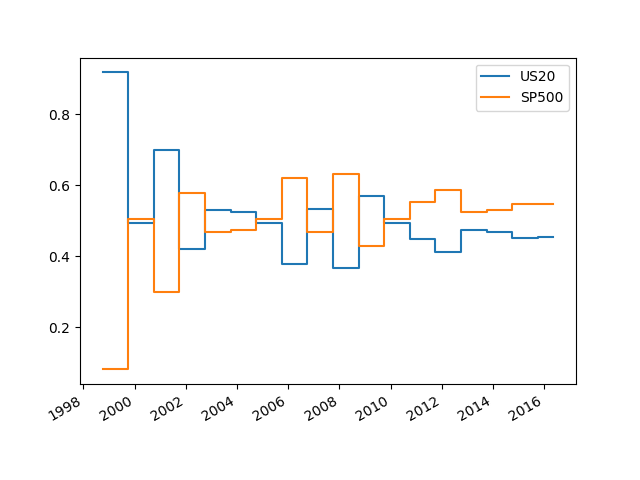
\includegraphics[height=8cm]{tser_voltar_01.png}

Enstruman Çeşitlendirme Çarpanı (Instrument Diversification Multiplier - IDM)

Tekrar üzerinden geçersek, risk hedeflememizi yaptık, her alt sistem içine bu
hedefe göre strateji doldurduk ki her alt sistem aynı riske sahip, ardından alt
sistem ağırlıklarını hesapladık ve her alt sisteme gerekli parayı ayırdık. Fakat
bu noktada ortaya bir problem çıkar, çünkü ağırlık kullanımı, ve alt sistem
getirilerinin arasında (elimizden geldiğince) korelasyonu az tutmuş olmamız
sebebiyle nihai sistemin genel riski azaldı. Yani hedeflediğimiz riskten sapmış
olduk. Elde etmek istediğimiz risk sanki her alt sistemi kendi başına
işletiyormuş gibi elde edeceğimiz risk gibi olmalı. O zaman bize öyle bir çarpan
lazım ki risk azalmasını telafi etsin, ve pozisyon hesabını yaparken bu çarpanı
uygulayarak risk hedefine geri dönelim.

N tane alt sistemimizin olduğunu düşünelim, bu sistemlerin getirilerinin
korelasyon matrisi $H$ olsun, ve biraz önce bulduğumuz ağırlıklar $W$ (ki
ağırlıkların toplamı 1). O zaman IDM, $1 / \sqrt{(W \cdot H \cdot W^T)}$
olacaktır. Dikkat edersek bu formül (2)'nin tam tersi. 

\begin{minted}[fontsize=\footnotesize]{python}
H = df.corr()
H = H.clip(lower=0)
print 'Korelasyon'
print H
W = np.array([[0.34,  0.66]]) # ustteki sonuc
idm=1.0 / (float(np.dot(np.dot(W, H), W.transpose()))) **.5
print '\nIDM', idm
\end{minted}

\begin{verbatim}
Korelasyon
           US20     SP500
US20   1.000000  0.096425
SP500  0.096425  1.000000

IDM 1.29697910974
\end{verbatim}

Tahmin Çarpanlarını Hesaplamak

Her tahmin algoritmasi için eldeki {\em tüm} veriler üzerinde tahmin üretiriz,
yani her enstrüman verisi için tahmin üretip, tüm bu tahminleri birleştirip koca
bir zaman serisi oluştururuz (bu tekniğe havuzlama -pooling- ismi veriliyor), ve
bu serinin mutlak değerlerinin (absolute value) ortalamasını alırız.

\begin{minted}[fontsize=\footnotesize]{python}
import util, zipfile, pandas as pd

ewmacs = [(2,8),(4,16),(8,32),(16,64),(32,128),(64,256)]

for (fast,slow) in ewmacs: 
    with zipfile.ZipFile('legacycsv.zip', 'r') as z:
        res = []
        for x in  z.namelist():
            if '_price' in x:
                df = pd.read_csv(z.open(x), index_col=0,parse_dates=True )
                tmp = util.ewma(df.PRICE, fast, slow)
                res.append(tmp)

    tmp = pd.DataFrame(pd.concat(res))
    tmp.columns = ['forecast']
    target_abs_forecast = 10.
    tmp=tmp.abs().iloc[:,0]
    avg_abs_value=tmp.mean()    
    print 'ewma', slow,fast,'=', target_abs_forecast/avg_abs_value
\end{minted}

\begin{verbatim}
ewma 2 8 = 12.8587606411
ewma 4 16 = 8.91499507015
ewma 8 32 = 6.09843054736
ewma 16 64 = 4.17115322451
ewma 32 128 = 2.84127283125
ewma 64 256 = 1.92365849221
\end{verbatim}

Taşıma kuralı (carry) için (not: TK verisini ayrı kontratlardan nasıl
yaratabileceğimizi {\em Vadeli İşlem Sözleşmeleri} bölümünde görmüştük, bu
yazıda basitlik amacı ile [1] için yaratılmış hazır veriyi kullanıyoruz),

\begin{minted}[fontsize=\footnotesize]{python}
import util, zipfile
import pandas as pd

with zipfile.ZipFile('legacycsv.zip', 'r') as z:
    res = []
    for x in z.namelist():
        if '_carrydata' in x:
            df = pd.read_csv(z.open(x), index_col=0,parse_dates=True )
            f = x.replace("__carrydata","_price")
            dfc = pd.read_csv(z.open(f),index_col=0,parse_dates=True )     
            vol = util.robust_vol_calc(dfc.PRICE.diff())
            carryoffset = np.abs(float((df.PRICE_CONTRACT - df.CARRY_CONTRACT).tail(1)))
            forecast =  util.carry(df.CARRY-df.PRICE, vol,np.abs(carryoffset)/12)
            res.append(forecast)

    tmp = pd.DataFrame(pd.concat(res))
    tmp = tmp.dropna()
    tmp.columns = ['forecast']
    tmp=tmp.abs().iloc[:,0]
    avg_abs_value=tmp.mean()
    print 10./avg_abs_value 
\end{minted}

\begin{verbatim}
21.44
\end{verbatim}

Bu değerler [1, sf. 309] ile uyumlu.

Strateji Ağırlıklarını Hesaplamak (Forecast Weight Estimation)

[1]'in yaklaşımlarından bir diğeri seçilen stratejilerin hangi ağırlıklarla her
alt sistem üzerinde kullanılacağını bulmak. Daha önce alt sistem içinde
stratejilere eşit ağırlık vermiştik. Gerçek dünyada bu ağırlıkların optimal
olması iyi olur. Her alt sistemde aynı strateji demeti olur, bu demetlere belli
ağırlıklar verilir, ve her alt sistem, aynı demeti bu ağırlıklar üzerinden
kullanır. Mesela petrol VİS'i üzerinde EWMAC 2,8, EWMAC 16,64 ve taşıma kuralı
(carry trade, TK) kullanıyor olabiliriz, bunların ağırlığı 0.2, 0.3, 0.5
olabilir. Diğer bir alt sistem, mesela kahve, Eurodollar aynı ağırlıkları aynı
şekilde kullanır.

Ağırlıkları bulmadan önce, hangi strateji demetiyle başlamak lazım? Bir liste
çıkartmak çok zor değil, [1, sf. 309]'a göre EWMAC'ın yavaş ve hızlı
parametreleri arasında 1'e 4 oranı mantıklı, yani EW 1,4, EW 2,8, EW 4,16, EW
8,32, diye devam edebiliriz. Bu listeden eleme yapmak için onların masraflarını
kullanmak iyi oluyor, çok masraflı olan stratejileri direk eleriz. Bu konuya
sonra döneceğiz.

Şimdilik nihai demeti kararlaştırmış olduğumuzu düşünelim, mesela CORN, EDOLLAR,
EUROSTX, MXP, US10, V2X üzerinde EW 16,64, EW 32,128, EW 64,256 ve TK
stratejilerini kullanacağız. Ağırlıkları hesaplamak için alt sistemler arası
kullandığımız hesaba benzer yaklaşımı kullanacağız, boostrap tekniğini devreye
sokacağız. Ayrıca havuzlama tekniğini de kullanacağız, eldeki {\em tüm}
enstrümanlar üzerinden elde edilen stratejilerin tahminlerini
birleştireceğiz. Mesela EWMAC 16,64 ile CORN, EDOLLAR, vs tahminleri yapıp bu
serileri uç uca koyacağız, böylece eldeki veriyi arttırmış olacağız.

\begin{minted}[fontsize=\footnotesize]{python}
import util, zipfile, pandas as pd, collections

ewmacs = [(16,64),(32,128),(64,256)]

forecasts = collections.OrderedDict()
for x in ewmacs: forecasts[x] = []
forecasts['carry'] = []
prices = collections.OrderedDict()
for x in ewmacs: prices[x] = []
prices['carry'] = []

insts = ['CORN', 'EDOLLAR', 'EUROSTX', 'MXP', 'US10', 'V2X']
with zipfile.ZipFile('legacycsv.zip', 'r') as z:
    for inst in insts: 
        df1 = pd.read_csv(z.open('%s_price.csv' % inst),\
                          index_col=0,parse_dates=True )     
        df2 = pd.read_csv(z.open('%s_carrydata.csv' % inst), \
                          index_col=0,parse_dates=True )     
        for (fast,slow) in ewmacs:
             vol = util.robust_vol_calc(df1.PRICE.diff())
             forecasts[(fast,slow)].append(util.ewma(df1.PRICE, fast, slow))
             prices[(fast,slow)].append(df1.PRICE)

        raw_carry = df2.CARRY_CONTRACT-df2.PRICE_CONTRACT
        carryoffset = df2.PRICE_CONTRACT - df2.CARRY_CONTRACT
        forecast =  util.carry(raw_carry, vol,  \
                               carryoffset*1/util.CALENDAR_DAYS_IN_YEAR)
        forecasts['carry'].append(forecast)
        prices['carry'].append(df1.PRICE)
    
for x in forecasts:
    forecasts[x] = pd.concat(forecasts[x])
for x in prices:
    prices[x] = pd.concat(prices[x])
    
dff = pd.DataFrame()
for x in forecasts: dff[x] = forecasts[x]
dfp = pd.DataFrame()
for x in prices: dfp[x] = prices[x]

rng = pd.date_range('1/1/1900', periods=len(dff), freq='D')

dff = dff.set_index(rng)
dfp = dfp.set_index(rng)

df = dfp.pct_change() * dff.shift(1)
df = df.dropna()
\end{minted}

\begin{minted}[fontsize=\footnotesize]{python}
import sys; sys.path.append('../tser_port')
import boot
weights=boot.optimise_over_periods(df, rollyears=20, monte_carlo=20,monte_length=250)
\end{minted}

Üstteki kod işledikten sonra EW 16,64, EW 32,128, EW 64,256, TK stratejileri
için sırayla 0.45, 0.05, 0.22, 0.28 ağırlıkları rapor edilecek. Bu değerler
[3]'te verilenlere benziyor, TK üzerinde oldukça ağırlık var, bu mantıklı
çünkü diğer stratejilerle çok korelasyonu olmayan bir strateji bu. Ortalama
hızdaki EWMA'ya yüzde 5 civarı verilmiş, geri kalanlar arasında daha hızlı
olan en çok ağırlığa sahip, değişimlere hızlı tepki verebilmenin faydası var
demek ki.

Stratejilerin Korelasyonu

Farklı EWMA stratejilerinin getirilerinin tek bir enstrüman üzerinden
korelasyonu altta bulunabilir [1, sf. 319]. 

\begin{minted}[fontsize=\footnotesize]{python}
import util, zipfile, pandas as pd, collections
ewmacs = [(2,8),(4,16),(8,32),(16,64),(32,128),(64,256)]
inst = 'US5'
with zipfile.ZipFile('legacycsv.zip', 'r') as z:
    p = pd.read_csv(z.open('%s_price.csv' % inst),\
                    index_col=0,parse_dates=True)
df = pd.DataFrame(index=p.index)
for (fast,slow) in ewmacs:
     fs = util.ewma(p.PRICE, fast, slow)
     df['%d-%d' % (fast,slow)] = util.ccy_returns(p.PRICE, fs)
print df.corr()
\end{minted}

\begin{verbatim}
             2-8      4-16      8-32     16-64    32-128    64-256
2-8     1.000000  0.869692  0.624934  0.402105  0.233632  0.143689
4-16    0.869692  1.000000  0.898819  0.673206  0.433222  0.270579
8-32    0.624934  0.898819  1.000000  0.902239  0.668067  0.437073
16-64   0.402105  0.673206  0.902239  1.000000  0.896226  0.657881
32-128  0.233632  0.433222  0.668067  0.896226  1.000000  0.891021
64-256  0.143689  0.270579  0.437073  0.657881  0.891021  1.000000
\end{verbatim}

Her stratejinin bir sonraki stratejiyle yakın bağlantısı olduğu görülüyor, ama
en azından bu bağlantı yüzde 99 değil, yüzde 90 civarı. 

Oynaklık Standardizasyonu 

Ornek: Bund beklenen getirisi yılda \%2\, beklenen yıllık standart sapma \%8.
Schatz vadeli işlem sözleşmesi 1\% ama beklenen oynaklık 2\%. Risk her iki
tarafta aynı olacak şekilde eşitleme yaparsak, Schatz'in beklenen getirisi
Bund'un iki katıdır.

\begin{minted}[fontsize=\footnotesize]{python}
import util

returns = [2.,1.] # bund,schatz
volatilies = [8.,2.] # bund,schatz
returns,vols = util.vol_equaliser(returns,volatilies)
print 'getiriler', returns
print 'oynaklik', vols
\end{minted}

\begin{verbatim}
getiriler [1.25, 2.5]
oynaklik [5.0, 5.0]
\end{verbatim}

Oynaklık standardizasyonu hesabı oynaklıklar için bir ortalama almaktan
ibarettir. Tüm oynaklıklar bu ortalamaya eşitlenir, ve aynı oranda
getiriler ayarlanır. 

Kaynaklar

[1] Carver, {\em Systematic Trading}

[2] Heydt, {\em Mastering Pandas for Finance}

[3] Carver, {\em Correlations, Weights, Multipliers.... }, \url{http://qoppac.blogspot.co.uk/2016/01/correlations-weights-multipliers.html}

\end{document}
